\chapter*{}

\begin{titlepage}
 
 
\setlength{\centeroffset}{-0.5\oddsidemargin}
\addtolength{\centeroffset}{0.5\evensidemargin}
\thispagestyle{empty}

\noindent\hspace*{\centeroffset}
\begin{minipage}{\textwidth}
\centering
\vspace{3.3cm}
%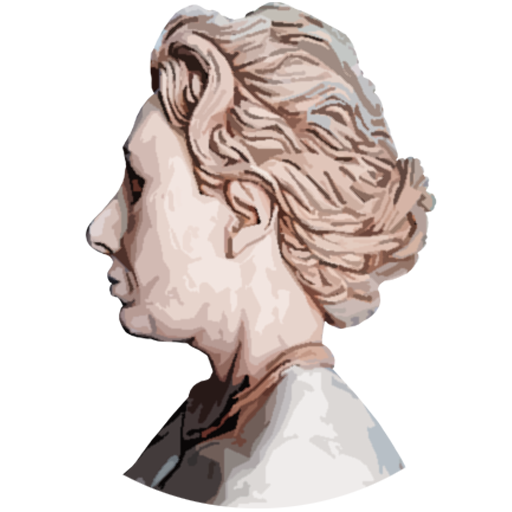
\includegraphics{imagenes/logo.png} 
%\vspace{0.5cm}

{\Huge\bfseries \myTitle \\}
\noindent\rule[-1ex]{\textwidth}{3pt}\\[3.5ex]
{\large\bfseries \mySubtitle \\[4cm]}
\end{minipage}

\vspace{2.5cm}

\noindent\hspace*{\centeroffset}
\begin{minipage}{\textwidth}
\centering
\textbf{Autor}\\ {\myName}\\[2.5ex]
\textbf{Director}\\ {\myProf}\\[2cm]
\end{minipage}

\vspace{\stretch{2}}

\end{titlepage}




\cleardoublepage
\thispagestyle{empty}

\begin{center}
{\large\bfseries \myTitle: \mySubtitle}\\
\end{center}

\begin{center}
\myName \\
\end{center}

\vspace{0.7cm}
\noindent{\textbf{Palabras clave}: informática gráfica, renderizado de volúmenes, tomografía computarizada, escultura policromada de madera, conservación y restauración, restaurador de arte}\\

\vspace{0.7cm}
\noindent{\textbf{Resumen}}\\

El objetivo principal de este proyecto es desarrollar un software diseñado para la documentación de datos volumétricos de esculturas policromadas de madera obtenidos mediante una Tomografía Computarizada (TC). El uso de esta técnica no destructiva permite a los expertos examinar el estado de la escultura de una manera más exhaustiva que usando la radiografía tradicional, la cual presenta limitaciones como la superposición de planos. La mayor parte de herramientas de renderizado volumétrico son muy caras y están orientadas a datos médicos, lo que las hace poco útiles para los restauradores debido a su precio y sus opciones de renderizado enfocadas al cuerpo humano. El software desarrollado permite cargar imágenes DICOM y realizar operaciones de renderizado y documentación como tomar medidas o extraer cortes en cualquier orientación. Se ha utilizado VTK como librería gráfica de alto nivel para leer los datos DICOM y renderizar el volumen generado con estos y Qt como librería para la creación de la interfaz gráfica de usuario.

\thispagestyle{empty}

\cleardoublepage

\begin{center}
	{\large\bfseries \myTitle: \myEnglishSubtitle}\\
\end{center}

\begin{center}
	\myName \\
\end{center}

\vspace{0.7cm}
\noindent{\textbf{Keywords}: Computer Graphics, Volume Rendering, Computed Tomography, Polychromed Wood Sculpture, Conservation-Restoration of Cultural Heritage, Art Curator}\\

\vspace{0.7cm}
\noindent{\textbf{Abstract}}\\

The main objective of this project is to develop a new software designed for the 3D documentation of polychromed wood sculptures from Computer Tomography (CT) datasets. This nondestructive technique allows experts to examine the artwork in a more confident and exhaustive manner than using the traditional X-ray plate which presents some limitations such as overlapping planes. Most of current available volume rendering tools are very expensive and orientated towards medical datasets, which makes unusable by art curators due to its price and its human-focused rendering options. The developed software loads DICOM files and performs rendering operations and several documentation actions, such as taking measurements or extracting slices at any orientation. It makes use of VTK as high-level graphics library for reading DICOM data and rendering the obtained volume and Qt as graphic user interface library.


\chapter*{}
\thispagestyle{empty}

\noindent\rule[-1ex]{\textwidth}{2pt}\\[4.5ex]

Yo, \textbf{\myName}, alumno de la titulación \myDegree de la \textbf{\myFaculty}, con DNI 75926571Y, autorizo la ubicación de la siguiente copia de mi Trabajo Fin de Grado en la biblioteca del centro para que pueda ser consultada por las personas que lo deseen.

\vspace{6cm}

\noindent Fdo: \myName

\vspace{2cm}

\begin{flushright}
\myLocation a \myTime.
\end{flushright}


\chapter*{}
\thispagestyle{empty}

\noindent\rule[-1ex]{\textwidth}{2pt}\\[4.5ex]

D. \textbf{\myProf}, Profesor del Área de Lenguajes y Sistemas Informáticos del \myDepartment de la \myUni.

\vspace{0.5cm}

\textbf{Informa:}

\vspace{0.5cm}

Que el presente trabajo, titulado \textit{\textbf{\myTitle, \mySubtitle}}, ha sido realizado bajo su supervisión por \textbf{\myName}, y autorizamos la defensa de dicho trabajo ante el tribunal que corresponda.

\vspace{0.5cm}

Y para que conste, expiden y firman el presente informe en \myLocation a \myTime.

\vspace{1cm}

\textbf{El director:}

\vspace{5cm}

\noindent \textbf{\myProf}

\chapter*{Agradecimientos}
\thispagestyle{empty}

\vspace{1cm}

No podría empezar de otra manera que dedicando unas palabras de agradecimiento a mis padres. Han luchado por mi educación y hoy estarán orgullosos de mi tanto como yo de ellos.
\\

Gracias a Javier Melero, mi tutor, por haberme guiado y motivado durante todo el curso. Sin él esto no sería posible.
\\

Gracias a todos los familiares y amigos con los que me he desahogado cuando algo no salía y me han escuchado pese a, muchas veces, no tener ni idea de lo que les estaba contando.
\\

Gracias también a mis compañeros de clase que no solo me han escuchado sino que también me han propuesto soluciones a problemas que surgían.
\\

Y como no, a \textit{Los Hijos de Vuctir} que me han acompañado durante estos cuatro años y han hecho más llevaderos los días de clase. No solo me llevo conocimientos de la universidad, también me llevo grandes amigos que pueden contar conmigo para lo que sea.